% =====================================================================
%  線上影音串流平台之二維動態策略模型 — 課程簡報 (Beamer, ENHANCED)
%  依使用者 guideline (IEGT final project slide.pdf) 重製:
%    格紙背景 + 寶藍 #003EA8 + 筆刷 + 彈簧線圈 + 星號;6 章節結構。
%  文獻經 workflow 上網查證 (見 RESEARCH_dossier.md);模型經 value iteration 求解 (06_enhanced_model.py)。
%  Engine: XeLaTeX  ·  Build: xelatex OTT_enhanced_slides.tex  (跑兩次)
% =====================================================================
\documentclass[aspectratio=169,11pt,fontset=none]{ctexbeamer}
\setCJKmainfont{PingFang TC}
\setCJKsansfont{PingFang TC}
\setCJKmonofont{Heiti TC}

\usepackage{amsmath,amssymb}
\usepackage{pifont}
\usepackage{tikz}
\usetikzlibrary{decorations.pathmorphing,positioning,arrows.meta}
\usepackage{graphicx}
\graphicspath{{./}}

% ---------- palette (sampled from the guideline deck) ----------
\definecolor{rblue}{HTML}{003EA8}
\definecolor{rblue2}{HTML}{1E5BD6}
\definecolor{gridc}{HTML}{DCE3F2}
\definecolor{ottred}{HTML}{E63946}
\definecolor{ottorange}{HTML}{F4A261}
\definecolor{ottteal}{HTML}{2A9D8F}
\definecolor{ottdark}{HTML}{264653}
\definecolor{ottsand}{HTML}{E9C46A}
\definecolor{ottgray}{HTML}{6B7B82}

\usetheme{default}
\useinnertheme{circles}
\setbeamertemplate{navigation symbols}{}
\setbeamercolor{structure}{fg=rblue}
\setbeamercolor{itemize item}{fg=rblue}
\setbeamercolor{itemize subitem}{fg=rblue2}
\setbeamercolor{enumerate item}{fg=rblue}
\setbeamercolor{block title}{fg=white,bg=rblue}
\setbeamercolor{block body}{fg=black,bg=rblue!7}
\setbeamercolor{block title alerted}{fg=white,bg=ottred}
\setbeamercolor{block body alerted}{fg=black,bg=ottred!8}
\setbeamercolor{block title example}{fg=white,bg=ottteal}
\setbeamercolor{block body example}{fg=black,bg=ottteal!9}
\setbeamerfont{frametitle}{series=\bfseries,size=\LARGE}
\setbeamerfont{block title}{series=\bfseries}

% ---------- clean, content-focused theme: plain white, no decorations ----------
\setbeamertemplate{background}{}                 % plain white (no grid/decorations)

% frame title: bold blue + thin rule underline
\setbeamertemplate{frametitle}{%
  \vskip0.55em
  {\usebeamerfont{frametitle}\color{rblue}\insertframetitle\par}%
  \vskip2pt{\color{rblue!40}\rule{\textwidth}{0.9pt}}\par\vskip0.15em}

% footer: compact 6-section progress bar, current section in bold blue
\setbeamertemplate{footline}{%
  \vskip1pt{\color{rblue!20}\hrule height0.4pt}\vskip2pt%
  \hbox to\paperwidth{\hskip1.1em\scriptsize
    \foreach \i/\nm in {1/背景動機,2/文獻回顧,3/模型建構,4/求解結果,5/延伸模型,6/結論}{%
      \ifnum\value{section}=\i\relax \textcolor{rblue}{\bfseries\nm}%
      \else \textcolor{black!35}{\nm}\fi
      \ifnum\i<6\relax\ \textcolor{black!20}{\textbar}\ \fi
    }%
    \hfill\textcolor{black!45}{\insertframenumber}\hskip1.1em}%
  \vskip2.5pt}

% small helpers
\newcommand{\chip}[1]{\tikz[baseline=-0.5ex]\node[fill=#1,inner sep=2.6pt,rounded corners=1pt]{};}
\newcommand{\hl}[1]{{\color{rblue}\bfseries #1}}
\newcommand{\mhl}[1]{{\color{rblue}#1}}   % math-safe highlight (no \bfseries)
\newcommand{\paper}[2]{\textbf{#1}\,{\footnotesize\color{ottgray}(#2)}}
% one-line reference:  **Author (Year)** (Venue) — explanation
% two-line reference:  **Author (Year)** (Venue):  /  gray plain-language result
\newcommand{\refx}[3]{\textbf{#1}\;{\color{ottgray}(#2)}:\\[1pt]{\color{ottgray}#3}\par\smallskip}
\newcommand{\refxn}[2]{\textbf{#1}:\\[1pt]{\color{ottgray}#2}\par\smallskip}

\title{線上影音串流平台之二維動態策略模型}
\author{Group E:徐晢恆、李思嫺、陳奕廷、廖振翔}
\date{Information Economics and Game Theory $\cdot$ 2026}

\begin{document}

% ----------------------------- Title -----------------------------
\begin{frame}[plain]
  \vfill
  \centering
  {\color{rblue}\rule{0.82\textwidth}{1.4pt}}\\[1.0em]
  {\fontsize{27}{32}\selectfont\bfseries\color{rblue} Two-Dimensional Dynamic Strategic Model\\[0.12em] for Online Video Streaming Platforms}\\[0.9em]
  {\LARGE\color{black!72} 線上影音串流平台之二維動態策略模型}\\[1.0em]
  {\color{rblue}\rule{0.82\textwidth}{1.4pt}}\\[1.8em]
  {\large\bfseries\color{black!75} Group E:徐晢恆\quad 李思嫺\quad 陳奕廷\quad 廖振翔}\\[0.6em]
  {\footnotesize\color{ottgray} Information Economics and Game Theory $\cdot$ 2026}
  \vfill
\end{frame}

% ----------------------------- TOC -----------------------------
\begin{frame}
  \vskip0.2em
  \begin{center}{\fontsize{27}{31}\selectfont\bfseries\color{rblue} Table of contents}\end{center}
  \vfill
  \begin{columns}[T]
    \column{0.5\textwidth}
      \large
      \textcolor{rblue}{\textbf{1.}}\enspace 研究背景與動機\\[1.1em]
      \textcolor{rblue}{\textbf{2.}}\enspace 文獻回顧\\[1.1em]
      \textcolor{rblue}{\textbf{3.}}\enspace 模型建構
    \column{0.5\textwidth}
      \large
      \textcolor{rblue}{\textbf{4.}}\enspace 求解結果與解讀\\[1.1em]
      \textcolor{rblue}{\textbf{5.}}\enspace 延伸模型與結果\\[1.1em]
      \textcolor{rblue}{\textbf{6.}}\enspace 結論
  \end{columns}
  \vfill
\end{frame}

% =====================================================================
\section{研究背景與動機}
% =====================================================================
\begin{frame}{研究背景與動機}
  市場上的影音串流(如 Netflix、Disney+),收費模式有兩種主要型態:
  \begin{itemize}
    \item \hl{單片租借制}(TVOD, Transactional Video on Demand)
    \item \hl{訂閱制}(SVOD, Subscription Video on Demand)
  \end{itemize}
  \vskip0.5em
  而在\textbf{客群策略}的維度可分為:
  \begin{itemize}
    \item \hl{新顧客獲取}(Acquisition):廣告投放、首月免費／優惠
    \item \hl{舊顧客留存}(Retention):演算法推薦優化、家庭方案、Bundle
  \end{itemize}
  \vskip0.6em
  \begin{block}{研究動機}
    這兩個維度都\textbf{與當前市佔率(Market Share)$s$ 密切相關}。本研究探討:廠商應如何\textbf{隨 $s$ 動態地}選擇收費模式與客群策略?
  \end{block}
\end{frame}

\begin{frame}{研究背景與動機－市場現有策略分析}
  \vskip0.8em
  \centering
  {\small\renewcommand{\arraystretch}{1.45}
  \begin{tabular}{l|l|l|l}
    \textbf{Platform} & \textbf{Market Share} & \textbf{Pricing} & \textbf{Customer strategy}\\\hline
    Netflix        & High          & Subscription  & Retention\\
    Disney+        & High to medium& Subscription  & Acquisition $\to$ Retention\\
    Apple TV+      & Low to medium & Subscription  & Acquisition\\
    YouTube Movies & Low           & Transactional & Acquisition\\
  \end{tabular}}
  \vskip1.0em
  \begin{flushleft}\footnotesize
  \textbf{觀察:}市佔率越高的平台越偏向\hl{訂閱制 + 留存};市佔率低的新進者偏向\hl{租借制／獲取}。
  Disney+ 隨市佔成長,策略由「獲取」轉向「留存」。
  \end{flushleft}
\end{frame}

\begin{frame}{研究問題}
  影音串流平台兩個維度的核心策略,都與當前市佔率 $s$ (Market Share)密切相關:
  \begin{columns}[t]
    \column{0.5\textwidth}\begin{block}{收費模式 $P$}\footnotesize
      \textbf{S} = 訂閱制 SVOD(Netflix 月費)\\
      \textbf{T} = 單部購買 TVOD(YouTube Movies 單片租購)\end{block}
    \column{0.5\textwidth}\begin{block}{客群策略 $C$}\footnotesize
      \textbf{A} = 新客獲取(廣告、試用)\\
      \textbf{R} = 舊客留存(推薦、折扣、內容)\end{block}
  \end{columns}
  \vskip0.2em
  \begin{center}\small
  \begin{tabular}{c|cc}
     & $C=A$(獲取) & $C=R$(留存)\\\hline
    $P=T$(TVOD) & \chip{ottred}\ \textcolor{ottred}{\textbf{Trans-Acq}} & \chip{ottorange}\ \textcolor{ottorange}{\textbf{Trans-Ret}}\\
    $P=S$(SVOD) & \chip{ottteal}\ \textcolor{ottteal}{\textbf{Sub-Acq}} & \chip{ottdark}\ \textcolor{ottdark}{\textbf{Sub-Ret}}\\
  \end{tabular}\end{center}
  \begin{alertblock}{核心問題}
    給定 $s$,廠商應如何在 4 種組合 $(P,C)\in\{T,S\}\times\{A,R\}$ 中選擇,以最大化跨期折現利潤?最適策略如何\textbf{隨 $s$ 變化}?
  \end{alertblock}
\end{frame}

% =====================================================================
\section{文獻回顧}
% =====================================================================
\begin{frame}{文獻回顧－ Two Dimension}
  \footnotesize\vskip0.1em
  \textbf{\color{rblue}Dimension 1:收費模式選擇(SVOD vs TVOD)}\par\smallskip
  \refx{Balasubramanian, Bhattacharya \& Krishnan (2015)}{Marketing Science}{selling(類 SVOD)vs pay-per-use(類 TVOD):獨佔利後者、競爭利前者。}
  \refx{Rao (2015)}{Marketing Science}{無承諾下「買斷(類 TVOD)」與「租用(類 SVOD)」並存最適,間接價格歧視。}
  \smallskip
  \textbf{\color{rblue}Dimension 2:客群策略(Acquisition vs Retention)}\par\smallskip
  \refx{Ben Rhouma \& Zaccour (2018)}{Management Science}{動態規劃最佳化獲取與留存支出(電信 panel 實證)。}
  \refx{Reinartz, Thomas \& Kumar (2005)}{J.\ of Marketing}{獲取/留存資源最適配置隨顧客關係階段而異。}
\end{frame}

\begin{frame}{文獻回顧－模型模板}
  \scriptsize\setlength{\smallskipamount}{1pt}\vskip0.1em
  \textbf{\color{rblue}\footnotesize 方法論模板:市佔率為狀態 + Bellman/DP 求解}\par\vskip1pt
  \refx{Sethi (1983)}{Optimal Control Appl.\ \& Methods}{市佔率 $x\in[0,1]$ 為狀態、廣告為控制,求 optimal $u^*(x)$}
  \refx{Ovchinnikov, Boulu-Reshef \& Pfeifer (2014)}{Management Science}{顧客基數為狀態、離散時間 Bellman 動態規劃,最適獲取/留存支出隨狀態調整。}
  \vskip2pt
  \textbf{\color{rblue}\footnotesize 模型機制(網路外部性／規模成本)}\par\vskip1pt
  \refxn{Farrell \& Klemperer (2007)}{網路外部性＋轉換成本}
  \refxn{Min et al.\ (2016)／Blattberg \& Deighton (1996)}{獲取成本隨市佔率遞增、留存並無此效應。}
\end{frame}

% =====================================================================
\begin{frame}{文獻回顧－文獻缺口與本研究貢獻}
  \begin{columns}[T]
    \column{0.5\textwidth}\footnotesize
    \begin{block}{文獻缺口}
      \begin{itemize}\itemsep4pt
        \item \textbf{定價維度:}探討 SVOD vs TVOD 收費模式,但多數\textbf{未同時納入獲客／留客}決策。
        \item \textbf{客群維度:}最佳化 Acquisition vs Retention,但通常\textbf{假設收費模式固定}。
      \end{itemize}
    \end{block}
    \column{0.5\textwidth}\footnotesize
    \begin{exampleblock}{本研究貢獻}
      將\textbf{定價}與\textbf{客群}兩維度納入\textbf{同一個 Bellman 模型},並讓收費模式 $P$ \textbf{同時影響}留存 $\rho$ 與獲取 $\alpha$。\\[3pt]
      求解得到\textbf{隨市佔率 $s$ 變化的最優策略} $a^*(s)$ 
    \end{exampleblock}
  \end{columns}
\end{frame}

% =====================================================================
\section{模型建構}
% =====================================================================
\begin{frame}{模型建構－環境設定}
  \begin{columns}[t]
    \column{0.56\textwidth}\footnotesize
      \begin{itemize}
        \item 單一廠商;離散時間 $t=0,1,2,\dots$(一期為一策略週期)
        \item 折現利率$\beta\in(0,1)$,取 $\beta=0.95$
        \item 潛在市場標準化 $N\equiv1$;市佔率 $s_t\in[0,1]$
        \item 可被獲取的潛在客戶: $1-s_t$
      \end{itemize}
      \vskip0.4em
      每期同時選兩個維度
      \[ a_t=(P_t,C_t),\quad P_t\in\{\mathrm T,\mathrm S\},\ C_t\in\{\mathrm A,\mathrm R\} \]
      \[ \mathcal A=\{(\mathrm{T,A}),(\mathrm{T,R}),(\mathrm{S,A}),(\mathrm{S,R})\} \]
    \column{0.44\textwidth}
      \begin{block}{$2\times2$ action matrix}\centering\footnotesize
        \begin{tabular}{c|cc}
          & $C{=}A$ & $C{=}R$\\\hline
          $P{=}T$ & \chip{ottred} TA & \chip{ottorange} TR\\
          $P{=}S$ & \chip{ottteal} SA & \chip{ottdark} SR\\
        \end{tabular}\end{block}
  \end{columns}
\end{frame}

\begin{frame}{模型建構－單期決策流程}
  \vskip0.7em
  \begin{center}
  \resizebox{\textwidth}{!}{%
  \begin{tikzpicture}[
    font=\footnotesize,
    box/.style={rounded corners=4pt, draw=black!25, line width=0.9pt, fill=white,
                minimum width=2.6cm, minimum height=1.5cm, align=center, inner sep=3pt},
    act/.style={rounded corners=4pt, draw=rblue, line width=1.4pt, fill=rblue!8,
                minimum width=2.6cm, minimum height=1.5cm, align=center, inner sep=3pt},
    nxt/.style={rounded corners=4pt, draw=ottteal, line width=1.4pt, fill=ottteal!10,
                minimum width=2.6cm, minimum height=1.5cm, align=center, inner sep=3pt},
    ar/.style={-{Stealth[length=3mm,width=2.4mm]}, line width=1.1pt, draw=black!50}]
    \node[box] (a) at (0,0)    {看到期初市佔\\[2pt]$s_t$};
    \node[act] (b) at (3.4,0)  {\textbf{選擇策略}\\[2pt]$(P_t,C_t)$};
    \node[box] (c) at (6.8,0)  {獲得本期利潤\\[2pt]$\pi(s_t,a_t)$};
    \node[box] (d) at (10.2,0) {舊客流失\\[2pt]新客加入};
    \node[nxt] (e) at (13.6,0) {進入下一期\\[2pt]$s_{t+1}$};
    \draw[ar] (a)--(b); \draw[ar] (b)--(c); \draw[ar] (c)--(d); \draw[ar] (d)--(e);
  \end{tikzpicture}}
  \end{center}
  \vskip0.9em
  \begin{itemize}\footnotesize
    \item 先觀察市佔 $s_t$,再從 4 種策略擇一 $(P_t,C_t)$,賺取當期利潤後,經舊客流失與新客加入決定 $s_{t+1}$。
    \item $s_t$ 在當期決策時\textbf{給定},$s_{t+1}$ 則由本期策略\textbf{內生}形成。
  \end{itemize}
\end{frame}

\begin{frame}{模型建構－狀態轉移(市佔率)}
  \[ \boxed{\,s_{t+1}=\underbrace{\rho(a_t,s_t)}_{\text{retention rate}}\cdot s_t \;+\; \underbrace{\alpha(a_t,s_t)}_{\text{Acquisition}}\cdot(1-s_t)\,} \]
  \begin{itemize}
    \item 第一項 $\rho\,s$:本期留下的\textbf{既有客戶}(留存率 $\rho$)。
    \item 第二項 $\alpha(1-s)$:從\textbf{非用戶池} $1-s$ 獲取的新客(獲取率 $\alpha$)。
    \item 以上兩項 ($\rho, \alpha$) 皆會根據 action ($a$) 與 market share ($s$) 而有變動。
  \end{itemize}
\end{frame}

\begin{frame}{模型建構－市佔率以水桶為例}
  \[ \boxed{\,s_{t+1}=\underbrace{\textcolor{rblue}{\rho(a_t)\,s_t}}_{\text{留下的舊客}}\;+\;\underbrace{\textcolor{ottteal}{\alpha(a_t)(1-s_t)}}_{\text{加入的新客}}\,} \]
  \vskip0.4em
  \begin{center}
  \begin{tikzpicture}[font=\small]
    \fill[rblue!15] (0,0) rectangle (4,1.15);
    \draw[line width=1.4pt, draw=rblue!75] (0,0) rectangle (4,2.2);
    \draw[rblue!45, line width=0.8pt] (0,1.15)--(4,1.15);
    \node[rblue, font={\footnotesize\bfseries}] at (2,0.55) {目前用戶池 $s_t$};
    \draw[-{Stealth[length=3mm,width=2.4mm]}, line width=1.6pt, ottteal] (-3,1.62) -- (-0.05,1.62);
    \node[ottteal, font={\scriptsize\bfseries}, anchor=south] at (-1.5,1.74) {新客流入 $\alpha(a_t)(1-s_t)$};
    \draw[-{Stealth[length=3mm,width=2.4mm]}, line width=1.6pt, ottred] (4.05,0.5) -- (6.9,-0.35);
    \node[ottred, font={\scriptsize\bfseries}, anchor=south west] at (4.9,0.45) {舊客流失 $1-\rho(a_t)$};
    \node[ottteal, font={\scriptsize\bfseries}, anchor=north west] at (-3,-0.45) {Acquisition:讓更多水流進來};
    \node[ottdark, font={\scriptsize\bfseries}, anchor=north west] at (4.1,-0.75) {Retention:把桶子的破洞補小};
  \end{tikzpicture}
  \end{center}
  \vskip0.4em
\end{frame}

\begin{frame}{模型建構－顧客留存率(Retention Rate $\rho$)}
  \[ \boxed{\,\rho(P,C,s)=\underbrace{\rho_0}_{\text{base rate}}+\underbrace{\delta_P+\delta_C}_{\text{strategy diff}}+\mhl{\kappa_\rho\, s}} \]
  \begin{columns}[T]
    \column{0.46\textwidth}\centering\small
    \begin{tabular}{c|cc}
       & $C{=}R$ & $C{=}A$\\\hline
      $P{=}S$ & $\rho_0{+}\delta_S{+}\delta_R{+}\kappa_\rho s$ & $\rho_0{+}\delta_S{+}\kappa_\rho s$\\
      $P{=}T$ & $\rho_0{+}\delta_R{+}\kappa_\rho s$ & $\rho_0{+}\kappa_\rho s$\\
    \end{tabular}\\[0.4em]
    {\scriptsize $\rho_0{=}0.65,\ \delta_S{=}{+}0.105,\ \delta_R{=}{+}0.10,\ \kappa_\rho{=}0.08$}
    \column{0.54\textwidth}\footnotesize
    \begin{block}{Strategy $\Rightarrow$ Retention rate}
      \begin{itemize}\itemsep1pt
        \item $\delta_S{>}0$:訂閱(S)固定月費綁定、flat-rate bias 使客戶黏著 $\to$ 留存高於計次(T)。{\color{ottgray}Lambrecht \& Skiera 2006。}
        \item $\delta_R{>}0$:留存策略(推薦/原創)提升留存。{\color{ottgray}Ben Rhouma \& Zaccour 2018。}
        \item $\kappa_\rho s$:平台越大、內容/推薦/社群效用越高(\textbf{network externality})。{\color{ottgray}Katz--Shapiro 1985。}
      \end{itemize}
    \end{block}
  \end{columns}
\end{frame}

\begin{frame}{模型建構－顧客獲取率(Acquisition rate $\alpha$)}
  \[ \boxed{\,\alpha(P,C,s)=\underbrace{\alpha_0}_{\text{base rate}}+\underbrace{\tilde\delta_P+\tilde\delta_C}_{\text{strategy diff}}+\mhl{\kappa_\alpha\, s}} \]
  \begin{columns}[T]
    \column{0.46\textwidth}\centering\scriptsize
    \begin{tabular}{c|cc}
       & $C{=}R$ & $C{=}A$\\\hline
      $P{=}S$ & $\alpha_0{+}\tilde\delta_S{+}\kappa_\alpha s$ & $\alpha_0{+}\tilde\delta_S{+}\tilde\delta_A{+}\kappa_\alpha s$\\
      $P{=}T$ & $\alpha_0{+}\tilde\delta_T{+}\kappa_\alpha s$ & $\alpha_0{+}\tilde\delta_T{+}\tilde\delta_A{+}\kappa_\alpha s$\\
    \end{tabular}\\[0.4em]
    {\scriptsize $\alpha_0{=}0.10,\ \tilde\delta_T{=}{+}0.05,\ \tilde\delta_A{=}{+}0.15,\ \kappa_\alpha{=}0.20$}
    \column{0.54\textwidth}\footnotesize
    \begin{block}{Strategy $\Rightarrow$ Acquisition rate}
      \begin{itemize}\itemsep1pt
        \item $\tilde\delta_T{>}0$:計次(T)無訂閱承諾、門檻低 $\Rightarrow$ 拉新較易,惟其留存較差。{\color{ottgray}Datta et al.\ 2015:免費試用客戶 CLV $-59\%$。}
        \item $\tilde\delta_A{>}0$:獲取策略(行銷/補貼)提高拉新。{\color{ottgray}Ben Rhouma \& Zaccour 2018。}
        \item $\kappa_\alpha s$:平台越大、口碑/網路擴散越快(\textbf{network externality})。{\color{ottgray}Godes--Mayzlin 2004。}
      \end{itemize}
    \end{block}
  \end{columns}
\end{frame}

\begin{frame}{模型建構－Profit function}
  \[ \boxed{\,\pi(s,a)=\underbrace{R(s,P)}_{\text{每用戶收入}}\cdot\, s \;-\; \underbrace{C(C,s)}_{\text{行銷成本}}\,} \]
  \begin{itemize}
    \item $R(s,P)$ 為每用戶每期收入,\quad $R(s,P)\cdot s$ 為總收入
    \item $C(C,s)$ 為每期行銷成本,\textbf{隨市佔率 $s$ 變動}。
  \end{itemize}
  \vskip0.4em
  \begin{block}{trade-off}\footnotesize
    \textbf{短期 vs.\ 跨期}:同 pricing 下 Retention 短期成本低; 但 Acquisition 提高 $\alpha$、推升未來 $s$,有跨期利益。\\
  \end{block}
\end{frame}

\begin{frame}{模型建構－Revenue \& Cost function}
  \[ \boxed{\,R(s,\mathrm S)=p_S,\qquad R(s,\mathrm T)=p_T\,(\varphi_0+\varphi_1\, s),\quad \varphi_1>0\,} \]
  \begin{columns}[T]
    \column{0.5\textwidth}\footnotesize
    \textbf{SVOD($p_S$)：}固定月費。
    \column{0.5\textwidth}\footnotesize
    \textbf{TVOD($p_T(\varphi_0{+}\varphi_1 s)$)：}平台越大、受眾越大,人均購買頻率隨 $s$ 上升。
  \end{columns}
  \vskip0.35em
  \[ \boxed{\,C_A(s)=c_A\,(1+\lambda_A\, s),\qquad C_R(s)=c_R\,(1+\lambda_R\, s),\qquad \lambda_A>\lambda_R\,} \]
  {\footnotesize\textbf{$\lambda_A>\lambda_R$:}市場越飽和,獲取(A)成本隨市佔率\textbf{陡升}、留存(R)無此規模效應 (Min et al.\ 2016)。\par}
  \vskip0.3em
  \begin{block}{參數設計}\footnotesize
    收入:$p_S{=}15,\ p_T{=}5,\ \varphi_0{=}\varphi_1{=}0.5$(低 $s$ 時 $R(s,S)>R(s,T)$)。\quad
    成本:$c_A{=}1.2,\lambda_A{=}1.0$($C_A{:}\,1.2\!\to\!2.4$);\ $c_R{=}0.8,\lambda_R{=}0.3$($C_R{:}\,0.8\!\to\!1.04$)。
  \end{block}
\end{frame}

\begin{frame}{模型建構－Bellman equation與 Value iteration}
  \[ \boxed{\,V(s)=\max_{a\in\mathcal A}\big\{\,\pi(s,a)+\beta\,V(s'(s,a))\,\big\}\,},\quad s'=\rho(a,s)\,s+\alpha(a,s)(1-s) \]
  \begin{columns}[T]
    \column{0.5\textwidth}\footnotesize
    \begin{block}{Bellman function}
      市佔 $s$ 的最大折現價值 $V(s)$ $=$ \textbf{當期利潤} $\pi(s,a)$ $+$ \textbf{折現續值} $\beta V(s')$;每個 $s$ 在 4 個 action 中取 maximum。\\[3pt]
      $\beta\in(0,1) \Rightarrow$ 唯一解 $V^*$ 存在、value iteration 必收斂。
    \end{block}
    \column{0.5\textwidth}\footnotesize
    \begin{exampleblock}{Value Iteration}
      1. 於 $s\in\{0,0.0025,\dots,1\}$, $V_0{=}0$。\\
      2. $Q=\pi+\beta\,V_k(s')$,$V_{k+1}=\max_a Q$,以線性插值取 $V_k(s')$。\\
      3. $\lVert V_{k+1}-V_k\rVert_\infty<10^{-8}$ 停止。
    \end{exampleblock}
  \end{columns}
\end{frame}

% =====================================================================
\section{求解結果與解讀}
% =====================================================================
\begin{frame}{求解結果－ 各 Strategy 的優勢區間}
  最適策略 $a^*(s)$ 在模型下呈現\textbf{三段結構}:
  \begin{center}
  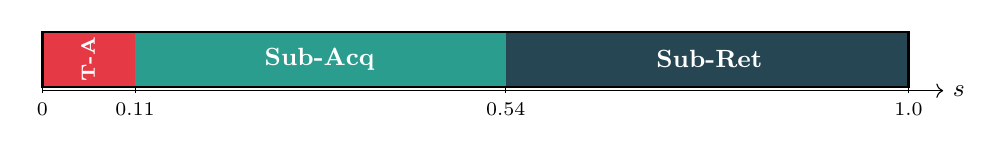
\begin{tikzpicture}[x=11cm,y=1cm]
    \fill[ottred](0,0)rectangle(0.107,0.7);\fill[ottteal](0.107,0)rectangle(0.535,0.7);\fill[ottdark](0.535,0)rectangle(1,0.7);
    \draw[thick](0,0)rectangle(1,0.7);
    \node[white,font=\scriptsize\bfseries,rotate=90]at(0.053,0.35){T-A};
    \node[white,font=\small\bfseries]at(0.32,0.35){Sub-Acq};
    \node[white,font=\small\bfseries]at(0.77,0.35){Sub-Ret};
    \draw[->](0,-0.05)--(1.04,-0.05)node[right]{\small $s$};
    \foreach \x in {0,0.107,0.535,1}\draw(\x,-0.02)--(\x,-0.08);
    \node[below,font=\scriptsize]at(0,-0.08){0};\node[below,font=\scriptsize]at(0.107,-0.08){0.11};
    \node[below,font=\scriptsize]at(0.535,-0.08){0.54};\node[below,font=\scriptsize]at(1,-0.08){1.0};
  \end{tikzpicture}
  \end{center}
  \centering\footnotesize
  \begin{tabular}{l|l|l}
    區間 & 策略 & 經濟意義\\\hline
    $s\in[0,0.11]$ & \textcolor{ottred}{\textbf{Trans-Acq}} & 新進市場;SVOD 短期虧損,TVOD 低門檻拉新客\\
    $s\in[0.11,0.54]$ & \textcolor{ottteal}{\textbf{Sub-Acq}} & 成長期; 透過 Acq 搶佔市場, SVOD 增加利潤\\
    $s\in[0.54,1]$ & \textcolor{ottdark}{\textbf{Sub-Ret}} & 成熟期; Ret 的網路外部性 $\kappa_\rho s$ 與規模成本使廠商保持策略\\
  \end{tabular}
  \vskip0.2em
  {\footnotesize $(T,R)$ 在任何 $s$ 都不會是最佳策略 — TVOD 較低人均收入使 Ret 策略在任何 $s$ 皆不划算。}
\end{frame}

\begin{frame}{求解結果－Steady State}
  \begin{columns}[T]
    \column{0.58\textwidth}\centering
      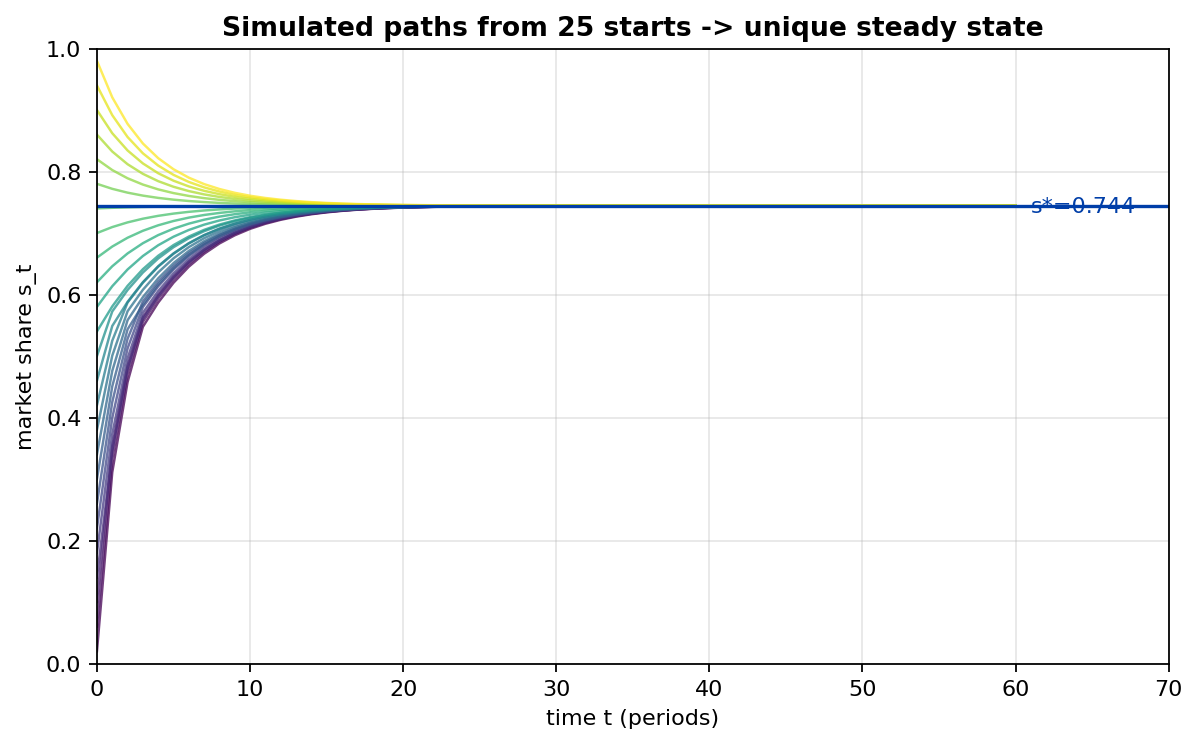
\includegraphics[width=\linewidth]{fig_value_paths.png}
    \column{0.42\textwidth}\footnotesize
      25 條不同起點 $s_0\in[0.02,0.98]$ 的模擬路徑\textbf{全部收斂到同一點}。
      \begin{alertblock}{唯一且全域收斂}
        $s_\infty\approx\mhl{0.744}$,\textbf{與起點無關}(無路徑相依)。
      \end{alertblock}
      \begin{block}{與實際情況的對比}\scriptsize
        $s_\infty\!\approx\!74\%$ 約等於\textbf{前 4-5 大 SVOD 合計}(66\%-78\%)，比照沒有競爭的情況。{\color{ottgray}(JustWatch US 2025Q4)}
      \end{block}
  \end{columns}
\end{frame}

\begin{frame}{求解結果－先進者優勢}
  \begin{columns}[T]
    \column{0.44\textwidth}\footnotesize
    \begin{itemize}\itemsep6pt
      \item 模擬三種起點:\textbf{新進}($s_0{=}0.05$)、\textbf{中型}($0.30$)、\textbf{大型}($0.65$)平台。
      \item 三者最後\textbf{收斂到同一穩態}($s_\infty\approx0.74$)——最終市佔一樣。
      \item 但\textbf{起點越高、25 年累積折現利潤越多};先發優勢來自\textbf{早期就坐擁高市佔}的那幾年。
    \end{itemize}
    \column{0.56\textwidth}\centering
    \vskip0.5em
    {\footnotesize
    \begin{tabular}{l|ccc}
      平台類型 & $s_0$ & 25期 $s$ & 25年折現利潤\\\hline
      \textcolor{ottred}{\textbf{Newcomer}} & 0.05 & 0.744 & 115.3\\
      \textcolor{ottteal}{\textbf{Mid-share}} & 0.30 & 0.744 & 124.3\\
      \textcolor{rblue}{\textbf{Incumbent}} & 0.65 & 0.744 & \textbf{141.8}\\
    \end{tabular}}\\[10pt]
    {\footnotesize 護城河 $=$ \textbf{絕對折現領先 $\approx 26.5$}(比值 ${\approx}23\%$ 會被折現分母稀釋,以絕對 gap 衡量較準)。}
  \end{columns}
\end{frame}

\begin{frame}{求解結果－ 留存/獲取率 隨 $s$ 的效益}
  \begin{columns}[T]
    \column{0.56\textwidth}\centering
      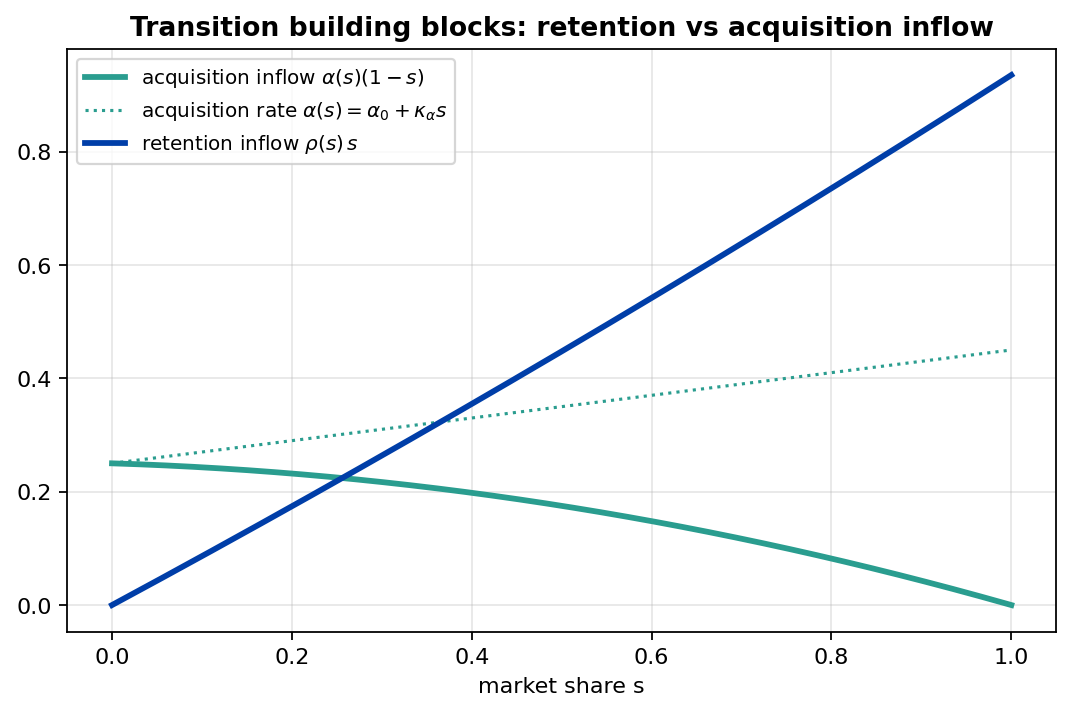
\includegraphics[width=\linewidth]{fig_buildingblocks.png}
    \column{0.44\textwidth}\footnotesize
      $s'=\rho(s)\,s+\alpha(s)(1-s)$ 可拆成兩股流入:
      \begin{itemize}\itemsep1pt
        \item \textbf{留存流入} $\rho(s)\,s$:隨 $s$ \textbf{凸增},由留存網路外部性 $\kappa_\rho$ 放大。
        \item \textbf{獲取流入} $\alpha(s)(1-s)$:隨 $s$ \textbf{遞減} —— 潛在客群 $(1-s)$ 枯竭壓過 $\kappa_\alpha$ 提升的人均獲取率。
      \end{itemize}
  \end{columns}
\end{frame}

\begin{frame}{求解結果－與現實世界的對應}
  \footnotesize
  \begin{block}{模型預測 $\leftrightarrow$ 現實觀察}
    \renewcommand{\arraystretch}{1.35}
    \begin{tabular}{p{0.46\textwidth}|p{0.48\textwidth}}
      \textbf{模型結果} & \textbf{現實對應}\\\hline
      低 $s$ 採 Trans-Acq(TVOD + 獲取) & YouTube Movies 以單片租購切入\\
      成長期 Sub-Acq(SVOD + 獲取) & Disney+、Apple TV+ 以訂閱 + 免費試用衝市佔\\
      成熟期 Sub-Ret(SVOD + 留存) & Netflix:推薦、原創, Disney+:後期推出 bundle\\
      Steady State $s_\infty$ 為 0.74 & 串流市場「強者恆強」、領導者市佔黏著\\
    \end{tabular}
  \end{block}
\end{frame}

% =====================================================================
\section{延伸模型與結果}
% =====================================================================
\begin{frame}{延伸模型1：臨界規模}
  {\footnotesize 在特定外生參數下,同一公司、同一套策略會走向\textbf{兩種長期結局},全看\textbf{起點規模}:\par}
  \vskip0.4em
  \begin{block}{觸發條件(兩者須同時)}\footnotesize
    \begin{itemize}\itemsep3pt
      \item \textbf{基礎留存 $\rho_0$ 低}(${\approx}0.3$):用戶易流失。
      \item \textbf{留存網路外部性 $\kappa_\rho$ 強}(${\gtrsim}0.5$):\textbf{用戶越多留存率越高}。
    \end{itemize}
  \end{block}
  \vskip0.45em
  \begin{center}
  \begin{tikzpicture}[font=\scriptsize]
    \draw[line width=1pt,-{Stealth[length=2.4mm]}] (0,0)--(10.5,0) node[right]{市佔 $s$};
    \foreach \x in {0,2.5,5,7.5,10}\draw[black!40](\x,-0.07)--(\x,0.07);
    \fill[rblue](5.33,0)circle(3pt); \node[below=2pt,rblue,font={\scriptsize\bfseries}]at(5.33,-0.06){0.53};
    \fill[rblue](9.4,0)circle(3pt); \node[below=2pt,rblue,font={\scriptsize\bfseries}]at(9.4,-0.06){0.93};
    \draw[ottred,line width=1.4pt](7.89,0.2)--(7.89,-0.2);
    \node[above=1pt,ottred,font={\scriptsize\bfseries}]at(7.89,0.22){臨界規模 0.79};
    \draw[ottteal,-{Stealth[length=1.8mm]},line width=1pt](3.0,0.45)--(4.4,0.45);
    \draw[ottteal,-{Stealth[length=1.8mm]},line width=1pt](7.2,0.45)--(6.0,0.45);
    \draw[ottteal,-{Stealth[length=1.8mm]},line width=1pt](8.5,0.45)--(9.1,0.45);
  \end{tikzpicture}
  \end{center}
  \vskip0.15em
  {\footnotesize\centering Starting State $s_0<0.79\Rightarrow$ 0.53;\quad $s_0>0.79\Rightarrow$ \textbf{0.93}。\par}
\end{frame}

\begin{frame}{延伸模型1：解讀}
  \begin{block}{結果詮釋}\footnotesize
    \begin{itemize}\itemsep4pt
      \item \textbf{小規模時}:用戶少、基礎留存率低 $\to$ 卡在低市佔。
      \item \textbf{衝過臨界規模}:黏性壓過流失、網路外部性 $\to$ 近乎獨佔。
    \end{itemize}
  \end{block}
  \vskip0.5em
  \begin{alertblock}{與現實的觀察和連接}\footnotesize
    \begin{itemize}\itemsep4pt
      \item 強網路效應平台的\textbf{贏者全拿}
      \item 串流大戰（或者是所有的市場）初期應投入資源搶佔市場(搶先過臨界規模)。
    \end{itemize}
  \end{alertblock}
\end{frame}

\begin{frame}{延伸模型2：競爭模型}
  \begin{columns}[T]
    \column{0.5\textwidth}\centering
    \vskip0.5em
    \begin{tikzpicture}[font=\scriptsize,
       box/.style={draw,rounded corners=3pt,minimum width=2.3cm,minimum height=1cm,align=center,line width=0.9pt}]
      \node[box,fill=rblue!12,draw=rblue] (N) at (0,1.7) {大公司\\$s_N$(黏)};
      \node[box,fill=ottred!12,draw=ottred] (C) at (4.6,1.7) {新進公司\\$s_C$(游移)};
      \node[box,fill=black!7,draw=black!45,minimum height=0.75cm] (U) at (2.3,-0.35) {未訂閱池 $U$};
      \draw[-{Stealth[length=2mm]},ottred,line width=1.1pt] (N) to[bend left=14] node[midway,above,font=\tiny,text=ottred]{挖 $\omega_N s_N$} (C);
      \draw[-{Stealth[length=2mm]},ottred,line width=1.1pt] (C) to[bend left=14] node[midway,below,font=\tiny,text=ottred]{挖 $\omega_C s_C$} (N);
      \draw[-{Stealth[length=1.8mm]},ottteal] (U)--(N) node[pos=0.55,left=-2pt,font=\tiny,text=ottteal]{$\alpha_N U$};
      \draw[-{Stealth[length=1.8mm]},ottteal] (U)--(C) node[pos=0.55,right=-2pt,font=\tiny,text=ottteal]{$\alpha_C U$};
    \end{tikzpicture}
    \par\vskip0.5em
    {\scriptsize\color{ottgray}\textbf{圖例}:\textcolor{ottred}{紅}$=$互挖對方游移客、\textcolor{ottteal}{綠}$=$從未訂閱池拉新。}
    \column{0.5\textwidth}\footnotesize
    \begin{block}{設定}
      \begin{itemize}\itemsep2pt
        \item 每期都有「游移客」$W{=}\omega s$ 可被對方挖;\textbf{新進公司客較游移} $\omega_C{=}0.15 > \omega_N{=}0.05$(大公司客\textbf{較黏})。
        \item 兩家也從\textbf{未訂閱池}拉新;大公司守留存、跌破 0.54 轉獲取。
      \end{itemize}
    \end{block}
    \vskip0.2em
    {\scriptsize $s_N'{=}\rho_N s_N+\alpha_N U-\alpha_C\omega_N s_N+\alpha_N\omega_C s_C$\par
     $s_C'{=}\rho_C s_C+\alpha_C U-\alpha_N\omega_C s_C+\alpha_C\omega_N s_N$\par
     {\color{ottgray}($\omega$ 即「對手專屬的流失率」,有效留存 $=\rho-\alpha_{\text{對手}}\omega$)}}
  \end{columns}
\end{frame}

\begin{frame}{延伸模型2：結果}
  \begin{columns}[T]
    \column{0.62\textwidth}\centering
      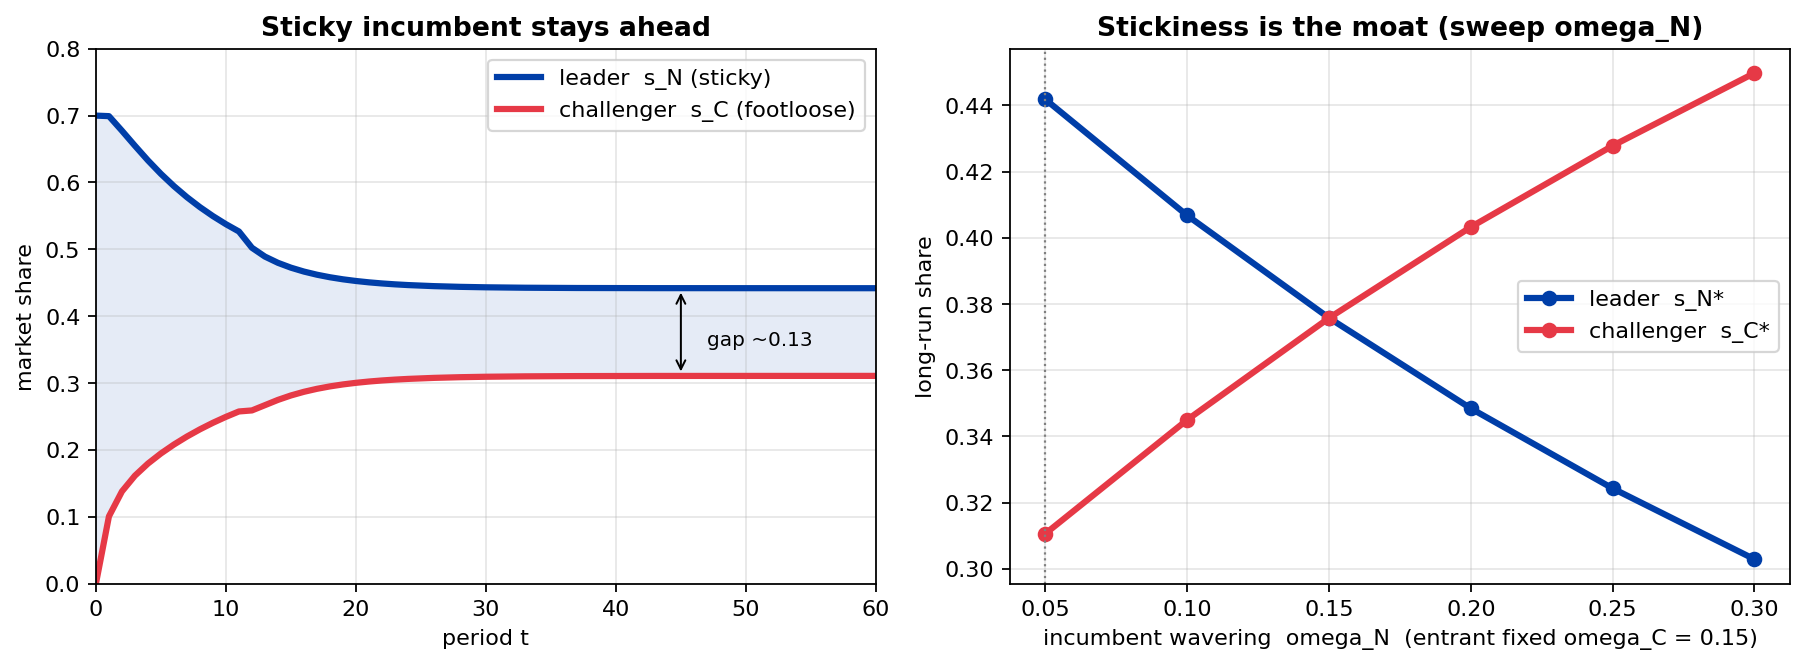
\includegraphics[width=\linewidth]{fig_ext3.png}
    \column{0.38\textwidth}\footnotesize
    \begin{block}{$\omega_N{=}0.05,\ \omega_C{=}0.15$}
      \begin{itemize}\itemsep3pt
        \item 大公司 $0.7\!\to\!\mathbf{0.44}$、新進公司 $0\!\to\!\mathbf{0.31}$(\textbf{被侵蝕但仍領先},gap ${\sim}0.13$)。
        \item \textbf{策略}:新進\textbf{全程獲取}(TA$\to$SA);大公司守\textbf{留存 SR}、跌破 0.54 轉獲取。
      \end{itemize}
    \end{block}
    \begin{exampleblock}{游移率對公司的影響}
      若大公司客也變游移($\omega_N\uparrow$):$\omega_N{=}0.05$ 領先、$0.15{=}$新進時\textbf{平手}、再高\textbf{被反超}。
    \end{exampleblock}
  \end{columns}
\end{frame}

\begin{frame}{延伸模型2:解讀}
  \footnotesize
  \begin{itemize}\itemsep5pt
    \item 大公司客低 $\omega$、新進客高 $\omega$;大公司\textbf{反挖}新進的游移客,守住領先。
    \item 一旦大公司\textbf{失去黏性}($\omega_N$ 升到 $\approx\omega_C$),領先就消失。
    \item 沒有游移($\omega{=}0$)新進幾乎打不進來($\sim$0.06)。
  \end{itemize}
  \vskip0.3em
  \begin{alertblock}{與現實的觀察和連接}\footnotesize
    解釋 Netflix 為何死守\textbf{降低顧客游移}(原創內容、個人化);市佔率不是唯一指標,更要看顧客的游移率。
  \end{alertblock}
\end{frame}

% =====================================================================
\section{結論}
% =====================================================================
\begin{frame}{結論－管理意涵}
  \footnotesize
  \begin{itemize}\itemsep4pt
    \item \textcolor{ottred}{\textbf{新進期(低 $s$):}}不宜一開始要求高承諾 —— 以\textbf{單部租購(TVOD)作為試水工具},低門檻先拉新。
    \item \textcolor{ottteal}{\textbf{成長期(中 $s$):}}不能只追求留存,否則\textbf{缺乏新客流入};須維持獲客動能。
    \item \textcolor{ottdark}{\textbf{成熟期(高 $s$):}}應\textbf{逐步將資源移向留存},但\textbf{不能完全停止獲客},以抵銷自然流失。
    \item \textcolor{rblue}{\textbf{網路效應強時:}}\textbf{早期跨越臨界規模}至關重要;落後臨界門檻恐困於低市佔均衡。
      \item \textcolor{ottorange}{\textbf{面對競爭時:}}市場已被大公司佔領時,\textbf{新進者}應專注\textbf{新客獲取}(挖游移客、搶未訂閱池);\textbf{在位者}則須\textbf{降低顧客游移率}(原創內容、防流失)以守住領先。
  \end{itemize}
\end{frame}

\begin{frame}{結論}
  \footnotesize
  \begin{enumerate}\itemsep2pt
    \item \textbf{三段策略地圖}:Trans-Acq $\to$ Sub-Acq $\to$ Sub-Ret 週期。
    \item \textbf{Dimension separation}:成本／網路效應主要移動\textbf{客群維度}($A/R$),收費維度($T/S$)由收入結構主導。
    \item \textbf{先進者優勢}:同穩態下先發者累積利潤領先 ${\approx}26.5$。
    \item \textbf{網路效應非單一方向}:留存外部性 $\kappa_\rho$ 鞏固龍頭、獲取口碑 $\kappa_\alpha$ 助挑戰者追趕。
    \item \textbf{延伸}:路徑相依僅在「低基礎留存＋高網路外部性」市場出現,小公司被擠進剩餘市場。
  \end{enumerate}
\end{frame}

\begin{frame}{References}
  \tiny
  \begin{columns}[T]
    \column{0.5\textwidth}
    \textbf{Balasubramanian, S., Bhattacharya, S., \& Krishnan, V.~V.} (2015). Pricing Information Goods: Selling vs.\ Pay-per-Use Mechanisms. \textit{Marketing Science}, 34(2).\par\smallskip
    \textbf{Ben Rhouma, T., \& Zaccour, G.} (2018). Optimal Marketing Strategies for the Acquisition \& Retention of Service Subscribers. \textit{Management Science}, 64(6).\par\smallskip
    \textbf{Blattberg, R.~C., \& Deighton, J.} (1996). Manage Marketing by the Customer Equity Test. \textit{Harvard Business Review}, 74(4).\par\smallskip
    \textbf{Datta, H., Foubert, B., \& Van Heerde, H.~J.} (2015). The Challenge of Retaining Customers Acquired with Free Trials. \textit{Journal of Marketing Research}, 52(2).\par\smallskip
    \textbf{Farrell, J., \& Klemperer, P.} (2007). Coordination and Lock-In: Competition with Switching Costs and Network Effects. \textit{Handbook of Industrial Organization}, Vol.\ 3.\par\smallskip
    \textbf{Godes, D., \& Mayzlin, D.} (2004). Using Online Conversations to Study Word-of-Mouth Communication. \textit{Marketing Science}, 23(4).\par\smallskip
    \textbf{Katz, M.~L., \& Shapiro, C.} (1985). Network Externalities, Competition, and Compatibility. \textit{American Economic Review}, 75(3).\par\smallskip
    \column{0.5\textwidth}
    \textbf{Lambrecht, A., \& Skiera, B.} (2006). Existence, Causes \& Consequences of Tariff-Choice Biases. \textit{Journal of Marketing Research}, 43(2).\par\smallskip
    \textbf{Min, S., Zhang, X., Kim, N., \& Srivastava, R.~K.} (2016). Customer Acquisition \& Retention Spending in Wireless Telecom. \textit{Journal of Marketing Research}, 53(5).\par\smallskip
    \textbf{Ovchinnikov, A., Boulu-Reshef, B., \& Pfeifer, P.~E.} (2014). Balancing Acquisition \& Retention Spending for Firms with Limited Capacity. \textit{Management Science}, 60(8).\par\smallskip
    \textbf{Rao, A.} (2015). Online Content Pricing: Purchase and Rental Markets. \textit{Marketing Science}, 34(3).\par\smallskip
    \textbf{Reinartz, W., Thomas, J.~S., \& Kumar, V.} (2005). Balancing Acquisition \& Retention Resources to Maximize Customer Profitability. \textit{Journal of Marketing}, 69(1).\par\smallskip
    \textbf{Sethi, S.~P.} (1983). Deterministic \& Stochastic Optimization of a Dynamic Advertising Model. \textit{Optimal Control Applications \& Methods}, 4(2).\par\smallskip
    \vskip0.4em
    {\color{ottgray}市場數據:JustWatch US Streaming Market Share, 2025 Q4。}
  \end{columns}
\end{frame}

\begin{frame}[plain]
  \vfill\centering
  {\color{rblue}\rule{0.5\textwidth}{1.4pt}}\\[0.8em]
  {\Large\bfseries\color{rblue} 謝謝聆聽}\\[0.6em]
  {\footnotesize\color{black!70} 線上影音串流平台之二維動態策略模型 $\cdot$ Group E}\\[0.6em]
  {\color{rblue}\rule{0.5\textwidth}{1.4pt}}
  \vfill
\end{frame}

\end{document}
